% Created 2016-08-17 Wed 14:38
\documentclass[tikz]{standalone}

\usepackage[utf8]{inputenc}
\usepackage[T1]{fontenc}
\usepackage{helvet}
\usepackage{../../templates/msc}

\renewcommand{\familydefault}{\sfdefault}

\tikzset{
every picture/.style={
line width=1pt
}}

\usepackage{tikz}
\author{Holger Karl}
\date{\today}
\title{}


\usetikzlibrary{positioning, fit, chains} 


\begin{document}
% \begin{tikzpicture}[auto, 
% block/.style = {rectangle, draw=black, thick, align=center},
% node distance = 0.5cm, 
% start chain= a going below]

%   \node[block, on chain]  {fixed\\sequencer};
%   \node[block, on chain]  {moving\\sequencer};
%   \node[block, on chain]  {privilege-\\based};
%   \node[block, on chain]  {communication \\history}; 
%   \node[block, on chain]  {destinations \\agreement}; 

%   \node (s1)  [left=of a-1] {Sequencer}; 
%   \node (s2) [left=of a-3] {Sender}; 
%   \node (s3) [left=of a-5] {Destinations}; 
  
%   \node[draw=red, fit = (s1) (a-1) (a-2)];

% \end{tikzpicture}
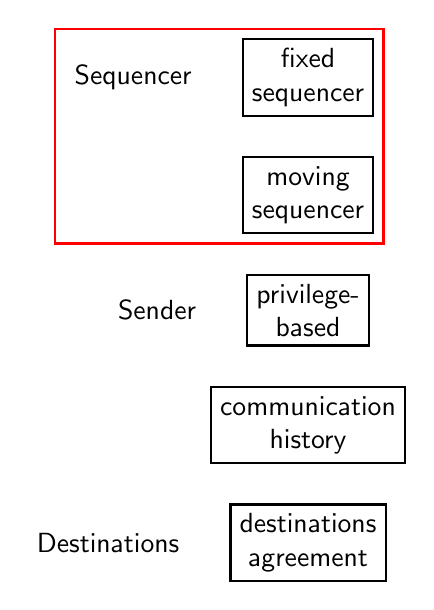
\begin{tikzpicture}[auto, 
block/.style = {rectangle, draw=black, thick, align=center},
node distance = 0.5cm, 
start chain= a going below]

  \node[block, on chain]  {fixed\\sequencer};
  \node[block, on chain]  {moving\\sequencer};
  \node[block, on chain]  {privilege-\\based};
  \node[block, on chain]  {communication \\history}; 
  \node[block, on chain]  {destinations \\agreement}; 

  \node (s1)  [left=of a-1] {Sequencer}; 
  \node (s2) [left=of a-3] {Sender}; 
  \node (s3) [left=of a-5] {Destinations}; 
  
  \node[draw=red, fit = (s1) (a-1) (a-2)] {};

\end{tikzpicture}
\end{document}